%
% Complete documentation on the extended LaTeX markup used for Insight
% documentation is available in ``Documenting Insight'', which is part
% of the standard documentation for Insight.  It may be found online
% at:
%
%     http://www.itk.org/

\documentclass{InsightArticle}

\usepackage[dvips]{graphicx}

%%%%%%%%%%%%%%%%%%%%%%%%%%%%%%%%%%%%%%%%%%%%%%%%%%%%%%%%%%%%%%%%%%
%
%  hyperref should be the last package to be loaded.
%
%%%%%%%%%%%%%%%%%%%%%%%%%%%%%%%%%%%%%%%%%%%%%%%%%%%%%%%%%%%%%%%%%%
\usepackage[dvips,
bookmarks,
bookmarksopen,
backref,
colorlinks,linkcolor={blue},citecolor={blue},urlcolor={blue},
]{hyperref}
\usepackage{subfig}


%  This is a template for Papers to the Insight Journal. 
%  It is comparable to a technical report format.

% The title should be descriptive enough for people to be able to find
% the relevant document. 
\title{Walk In A Triangulation : Straight Walk}

% 
% NOTE: This is the last number of the "handle" URL that 
% The Insight Journal assigns to your paper as part of the
% submission process. Please replace the number "1338" with
% the actual handle number that you get assigned.
%
\newcommand{\IJhandlerIDnumber}{1338} %TOMODIFY

% Increment the release number whenever significant changes are made.
% The author and/or editor can define 'significant' however they like.
\release{0.01}

% At minimum, give your name and an email address.  You can include a
% snail-mail address if you like.
\author{St\'{e}phane Rigaud$^{1}$ and Alexandre Gouaillard$^{2}$}
\authoraddress{$^{1}$Image \& Pervasive Access Lab, National Centre for Scientific Research (CNRS), Fusionopolis, Singapore\\
               $^{2}$Singapore Immunology Network, Agency for Science, Technology and Research (A*STAR), Biopolis, Singapore}

\begin{document}

%
% Add hyperlink to the web location and license of the paper.
% The argument of this command is the handler identifier given
% by the Insight Journal to this paper.
% 
\IJhandlefooter{\IJhandlerIDnumber}


\ifpdf
\else
   %
   % Commands for including Graphics when using latex
   % 
   \DeclareGraphicsExtensions{.eps,.jpg,.gif,.tiff,.bmp,.png}
   \DeclareGraphicsRule{.jpg}{eps}{.jpg.bb}{`convert #1 eps:-}
   \DeclareGraphicsRule{.gif}{eps}{.gif.bb}{`convert #1 eps:-}
   \DeclareGraphicsRule{.tiff}{eps}{.tiff.bb}{`convert #1 eps:-}
   \DeclareGraphicsRule{.bmp}{eps}{.bmp.bb}{`convert #1 eps:-}
   \DeclareGraphicsRule{.png}{eps}{.png.bb}{`convert #1 eps:-}
\fi


\maketitle


\ifhtml
\chapter*{Front Matter\label{front}}
\fi


% The abstract should be a paragraph or two long, and describe the
% scope of the document.
\begin{abstract}
\noindent
This document describes the implementation in ITK of the \emph{Straight Walk in a Triangulation} algorithm proposed by Devillers \emph{et al.} \cite{Devillers2001}. Using the \emph{exact discrete geometrical orientation predicate} \cite{Moreau2011}, and the \emph{itk::QuadEdgeMesh} API \cite{Gouaillard2006} of ITK , we propose an efficient implementation that locates a point in a triangulated mesh structure. This paper is accompanied with the source code and examples that should provide enough details for users.
This work has for principal intended an exact and robust implementation of a Delaunay triangulation / Voronoi tesselation in ITK, which will be presented in a separate paper, once done :).

% description of the principle and interest
% description of the algorithm
% description of the implementation
% validation, example and usage
% conclusion

\end{abstract}

\IJhandlenote{\IJhandlerIDnumber}

\tableofcontents

\section{Principle of Walking in a Triangulation}

Taking a triangulated mesh 2-manifold planar structure $\mathcal{T}$ of $\mathit{n}$ vertices embedded into a \emph{n}-dimensions space, and supposing that $\mathcal{T}$ has only one component and only one boundary,  we try to find the triangle $\mathit{t}$ of $\mathcal{T}$ that contain a given point $\mathit{p}$. One of the simplest and most effective strategy is the Straight Walk, which consists in, given a specific or random starting point $\mathit{q}$, going through all the triangles along the direction vector $\overrightarrow{\mathit{qp}}$, using adjacency relation between triangles until the triangle that contains the point $\mathit{p}$ is reached (Fig \ref{fig:straightwalka}).
This algorithm is especially used in Delaunay triangulation as it can be proved that it actually converges to the right triangle in a $\mathcal{O}(\lvert \mathit{qp}\rvert \sqrt{\mathit{n}})$ complexity, with $\mathit{n}$ the number of vertices of $\mathcal{T}$, and $\lvert\mathit{qp}\rvert$ the distance between $\mathit{q}$ and $\mathit{p}$.
The path followed by the Straight Walk is determined by an orientation predicate (simple geometric question) that gives us the direction to follow in the triangulation.

\section{Implementation}

The algorithm is implemented as a functor templated over the mesh type and the output type defined in \emph{itk::QEMeshFunctionBase}. It take in arguments a triangular mesh (\emph{itk::QuadEdgeMesh}), a point coordinate (\emph{itk::QuadEdgeMesh::PointType}) and optionally a starting triangle (\emph{itk::QuadEdgeMesh::CellIdentifier}). It returns a vector of index (\emph{itk::VectorContainer}) that contains the list of the visited triangles' identifiers. The last element of the vector is corresponding to the index of the triangle containing the input point.

From the given initial triangle $\mathit{t}$, we randomly determine $\mathit{q}$, one of the vertices of $\mathit{t}$. We rotate around $\mathit{q}$ until the current triangle incident to $\mathit{q}$ is intersecting with the $\overrightarrow{\mathit{qp}}$ vector. Once $\mathit{t}$ is intersecting with $\overrightarrow{\mathit{qp}}$, we test on witch edge $\mathit{e}$ the vector $\overrightarrow{\mathit{qp}}$ is going out of $\mathit{t}$ using the orientation predicate (Eq. \ref{predicate}). We move to the neighbour triangle of $\mathit{t}$ that share the edge $\mathit{e}$ and test again, in the new triangle, which edge is crossed by the $\overrightarrow{\mathit{qp}}$. The walk stops when no edge crossing $\overrightarrow{\mathit{qp}}$ is found (Fig \ref{fig:straightwalkb}).

\begin{equation} \label{predicate}
\mathit{orientation(\alpha, \beta, \gamma)} ~=~\mathit{sign} \left( \left\lvert
\begin{matrix}
\beta_{x}-\gamma_{x} & \alpha_{x}-\gamma_{x} \\
\beta_{y}-\gamma_{y} & \alpha_{y}-\gamma_{y}
\end{matrix}
\right\rvert \right)
\end{equation}

For robustness and exactness in the algorithm, the predicate is done by using the ITK implementation of an exact discrete geometrical predicate \cite{Moreau2011} based on the work of Shewchuk \cite{Shewchuk97a}.
For more details, please refer to the scientific article \textit{Walk in a Triangulation} \cite{Devillers2001}.

\begin{figure}
\center
\subfloat[]{\label{fig:straightwalka}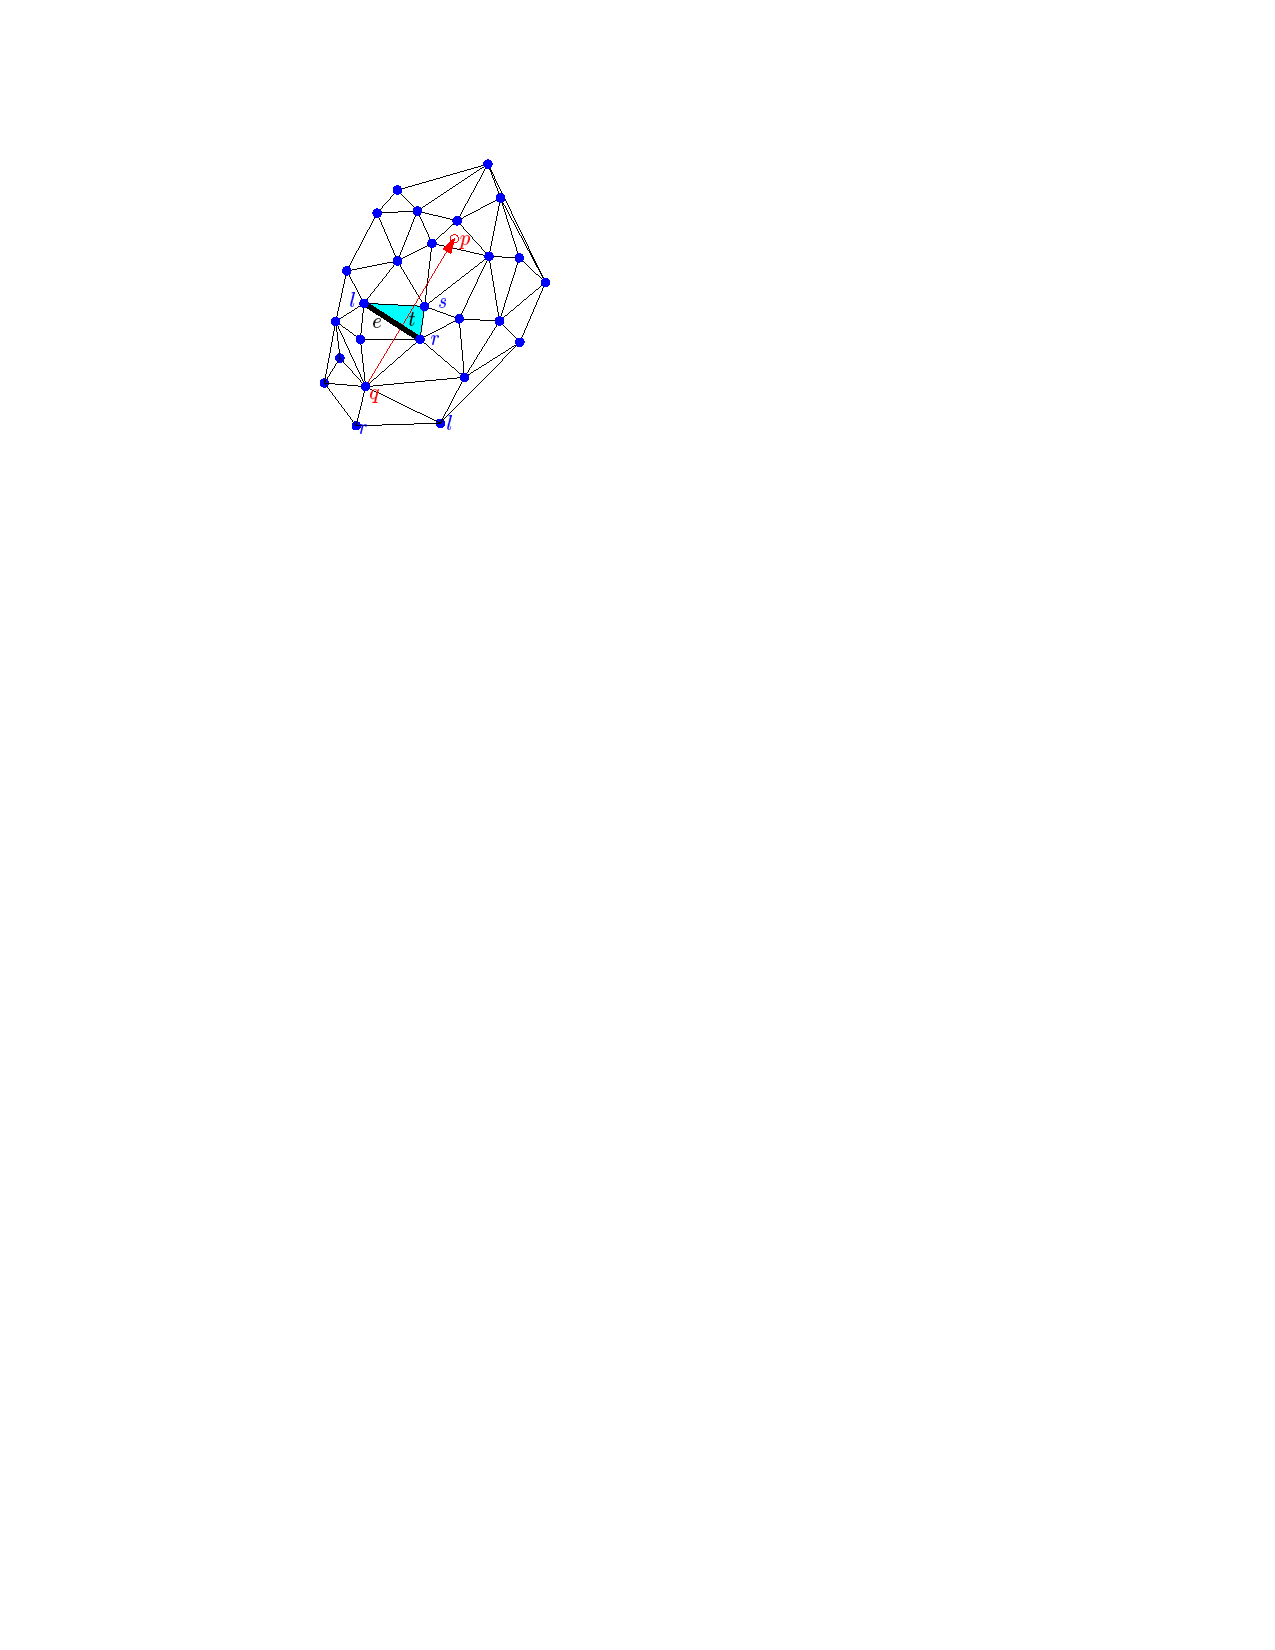
\includegraphics[width=0.35\textwidth]{Algorithm_description}} \hspace{10pt}
\subfloat[]{\label{fig:straightwalkb}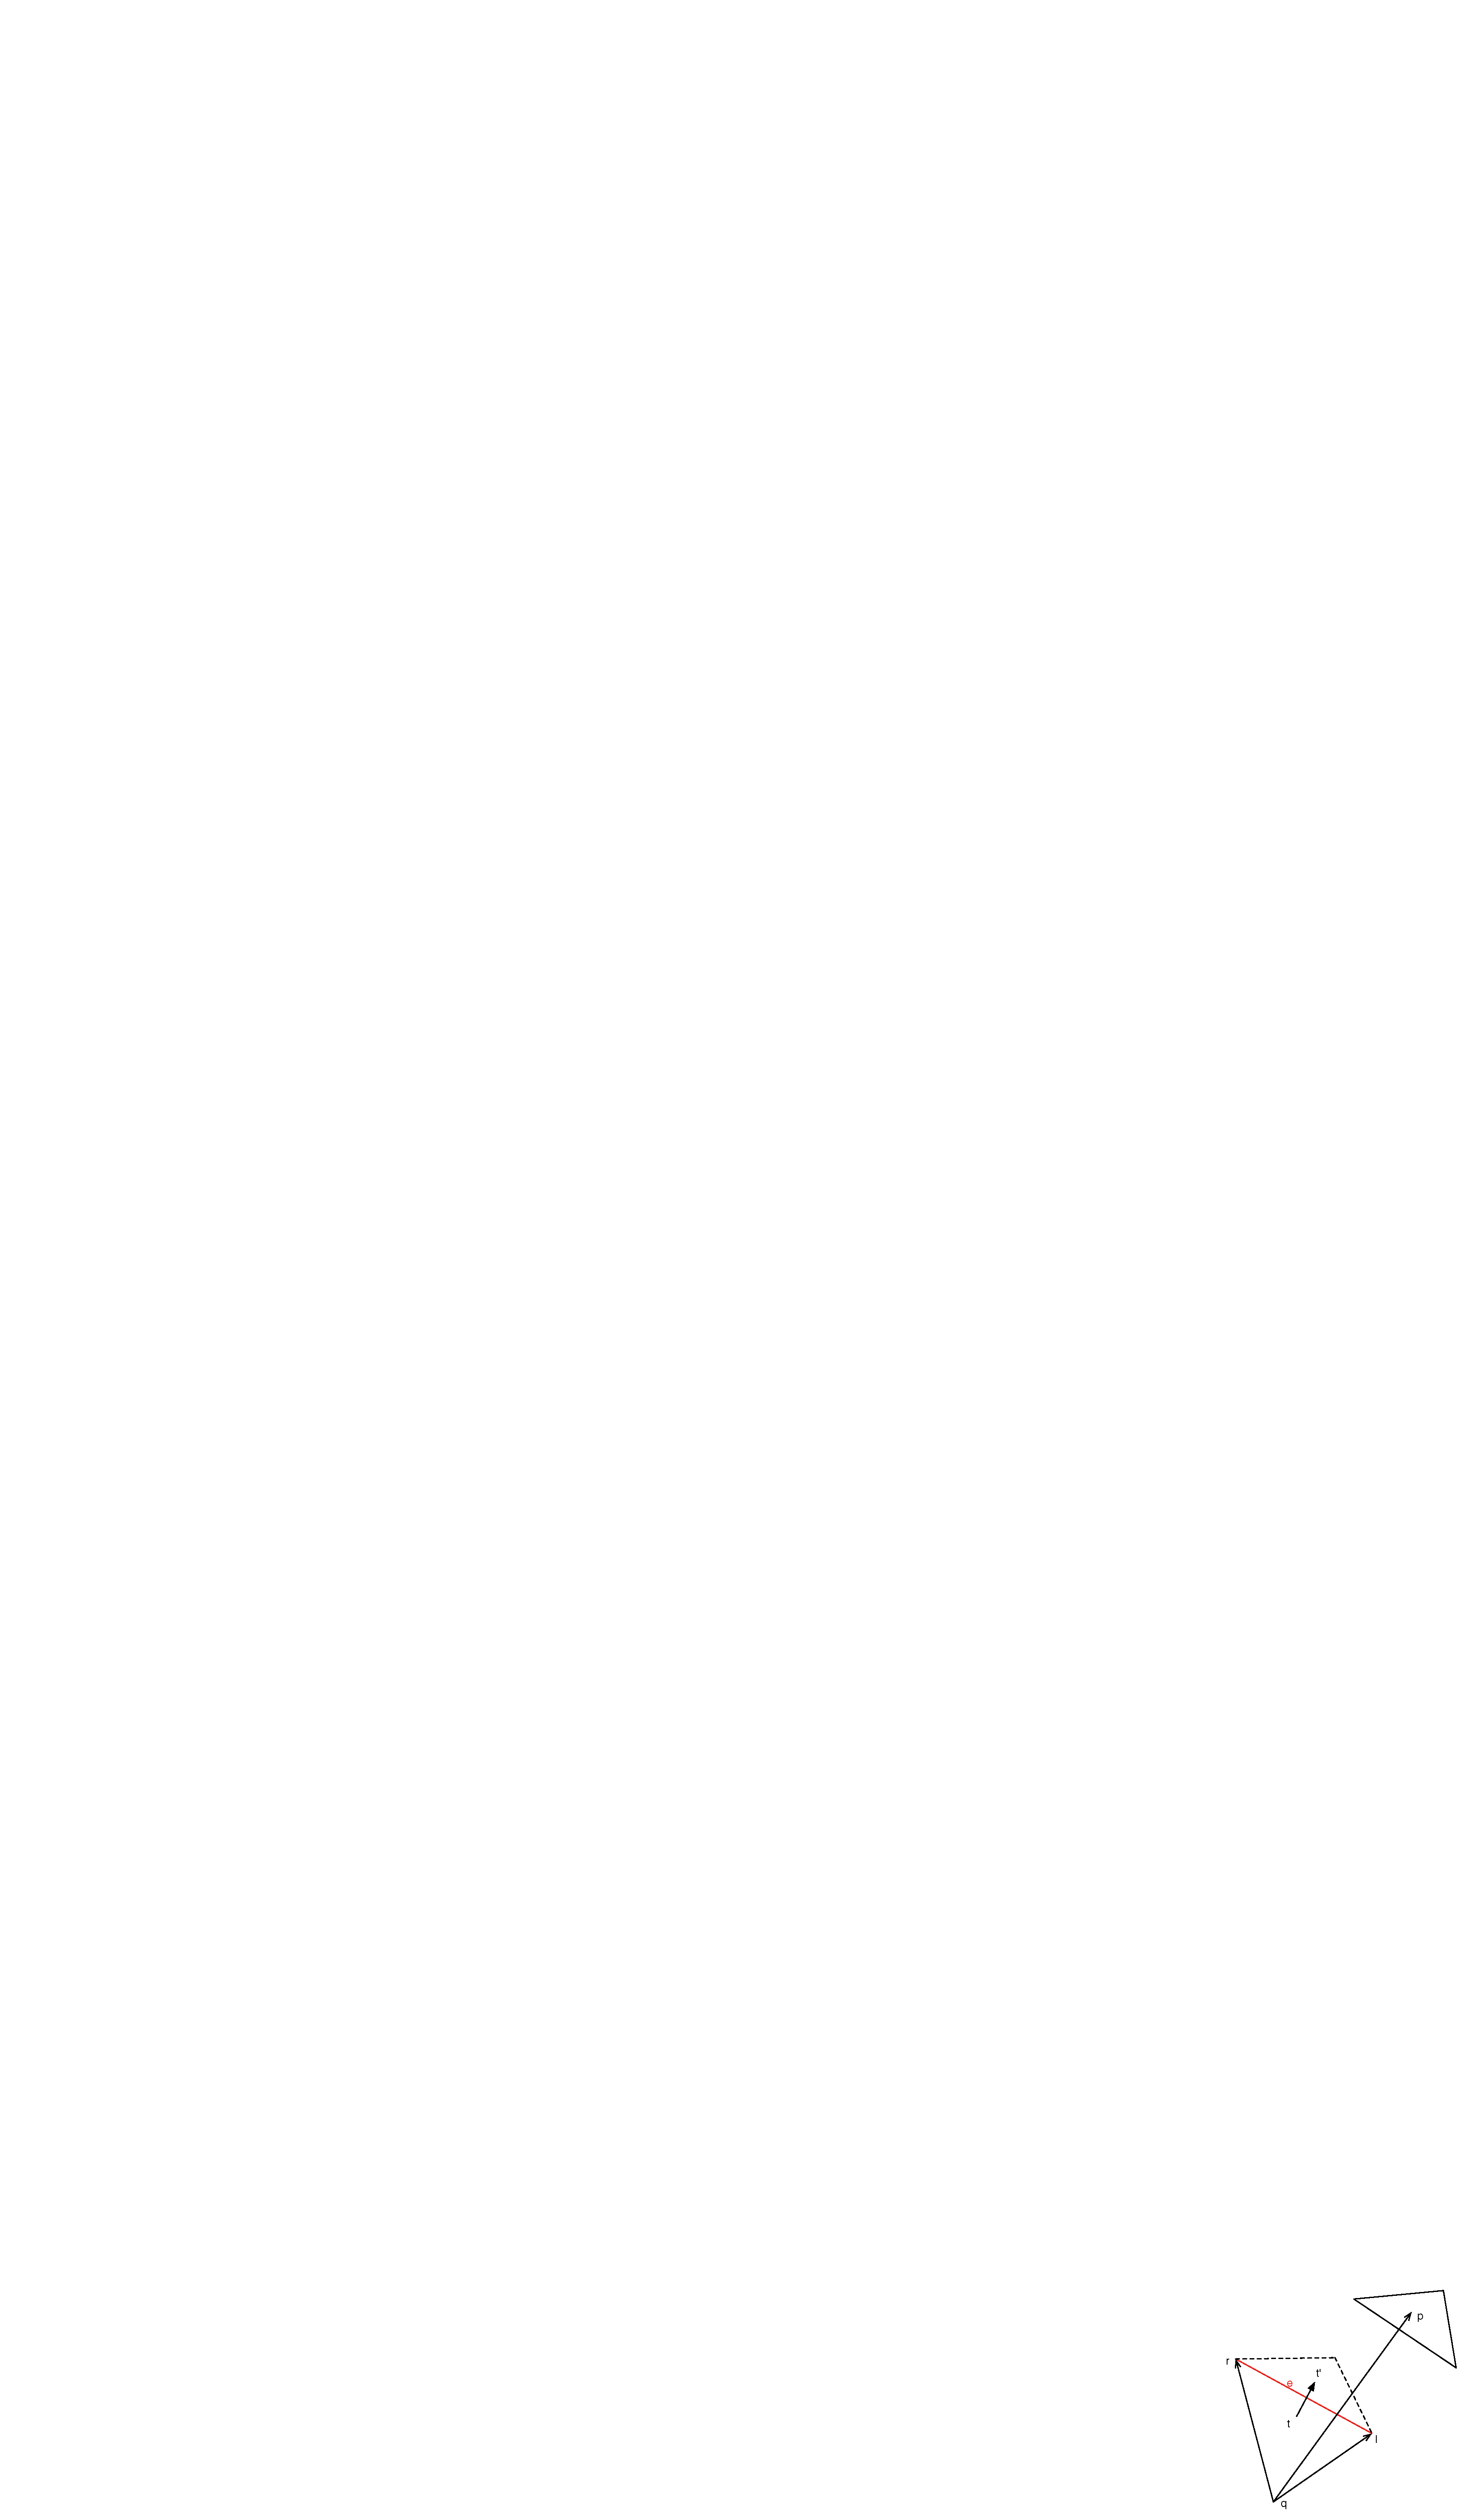
\includegraphics[width=0.35\textwidth]{Algorithm_predicate}}
\itkcaption{Straight Walk in a Triangulation Algorithm}
\label{fig:straightwalk}
\end{figure}

\section{Usage}

An example \texttt{WalkInTriangulation.cxx} is provided with the sources and is used for the tests. The functor is templated on 2 dimensions \textit{itk::QuadEdgeMesh}, if a higher dimensions mesh is given, only the two first dimension will be used in the process. The initialisation triangle is optional, if not specified the algorithm will start at the first triangle in the cell container.
\begin{verbatim}
itk::WalkInTriangulation< TQuadEdgeMesh, 
                          itk::VectorContainer<unsigned int, TCellIdentifier> >
( TQuadEdgeMesh *, TPointType &, TCellIdentifier & )
\end{verbatim}


%%%%%%%%%%%%%%%%%%%%%%%%%%%%%%%%%%%%%%%%%
%
%  Insert the bibliography using BibTeX
%
%%%%%%%%%%%%%%%%%%%%%%%%%%%%%%%%%%%%%%%%%

\bibliographystyle{plain}
\bibliography{InsightJournal}


\end{document}

